\section{Realtime Evidence}
\label{sec:evidence}

\begin{frame}{Realtime evidence}
  In principle the realtime evidence is based on four steps:
  \begin{enumerate}
    \item Evaluate the relevant characteristics of the technical process:
      \begin{enumerate}
        \item number of different requests,
        \item minimum processing time for each request,
        \item minimum allowable response time $T_{Z,min}$ for each request,
        \item maximum allowable response time $T_{Z,max}$ for each request,
        \item dependencies between events.
      \end{enumerate}
    \item Identify the maximum processing time $T_{V,max}$ (WCET, worst-case execution time) for each request.
    \item Check the load condition $\rho = T_V/T_P < 1$.
    \item Verify the timeliness condition: determine $T_{R,min}$ and $T_{R,max}$ and check $T_{Z,min} \le T_{R,min}$, $T_{R,max} \le T_{Z,max}$.
  \end{enumerate}
\end{frame}

\scriptonly{%
Step~4 is the hard part. The maximum response time $T_{R,max}$ contains the WCET of the request itself and the latency caused by everything that can delay it: other tasks, interrupts, and code that runs with interrupts disabled. All of these must be known as worst-case values, so the whole argument rests on the WCET of every code section.
}

\begin{frame}{WCET by measurement}
  \begin{itemize}
    \item Record time stamps $t_1$ (start) and $t_2$ (end) of the code section, for example with a port pin and a logic analyzer (Chapter~\ref{sec:timing}) or with the run-time counter (Chapter~\ref{sec:runtimestats}).
    \item Each run $i$ gives $T_{V,i} = t_2 - t_1$, and the result is $T_{V,max} = \max_i T_{V,i}$.
    \item The input values and events must be generated such that the worst case is actually hit, and the whole system must be under load (e.g.\ by an automatic tester).
  \end{itemize}
\end{frame}

\begin{frame}{Measurement: pros and cons}
  \begin{columns}[T]
    \begin{column}{0.42\textwidth}
      \textbf{Advantages}
      \begin{itemize}
        \item independent of the programming language
        \item relatively easy to implement
        \item can run as autonomous self-diagnosis
      \end{itemize}
    \end{column}
    \begin{column}{0.56\textwidth}
      \textbf{Disadvantages}
      \begin{itemize}
        \item no guarantee: the maximum seen is not necessarily the worst case (loops, branches, caches, interrupts)
        \item expensive: in theory all input combinations
        \item only on the target with running code, i.e.\ late in the project
        \item needs a test environment and modified code (time stamps)
        \item system load is hard to generate
      \end{itemize}
    \end{column}
  \end{columns}
  \medskip
  $\Rightarrow$ Look at what the processor actually executes: machine instructions and machine cycles.
\end{frame}

% ===========================================================================
\section{Program Execution on the Microcontroller}
\label{sec:machine}

\subsection{CPU and registers}
\begin{frame}{CPU components}
  \begin{center}
  \begin{tikzpicture}[x=1cm,y=1cm,>=Stealth,font=\footnotesize,
      box/.style={draw,fill=blue!10,minimum height=0.6cm,minimum width=1.5cm,align=center},
      mem/.style={draw,fill=orange!15,minimum height=3.0cm,minimum width=2.2cm,align=center}]
    \node[box] (pc)  at (0,2.7)   {PC};
    \node[box] (mar) at (2.4,2.7) {MAR};
    \node[box] (ir)  at (0,1.2)   {IR};
    \node[box] (gpr) at (3.2,1.2) {Registers\\ACC, B, R0--R7};
    \node[box] (sp)  at (5.4,1.2) {SP};
    \node[box,minimum width=2.4cm] (cu) at (0,0) {Control unit\\(decoder, FSM)};
    \node[box] (alu) at (3.2,0)   {ALU};
    \node[box] (ccr) at (5.4,0)   {PSW / CCR};
    \node[mem] (m)   at (8.6,1.35) {Program\\memory\\[2pt] Data memory\\[2pt] I/O, SFR};
    \draw[->,thick] (pc) -- (mar);
    \draw[->,thick] (mar) -- node[above]{address bus} (m.west |- mar);
    \draw[line width=2pt,gray] (-0.8,2.0) -- (m.west |- 0,2.0) node[pos=0.85,above,black]{data bus};
    \draw[->] (ir.north |- 0,2.0) -- (ir.north);
    \draw[<->] (gpr.north |- 0,2.0) -- (gpr.north);
    \draw[<->] (sp.north |- 0,2.0) -- (sp.north);
    \draw[->] (ir) -- (cu);
    \draw[<->] (gpr) -- (alu);
    \draw[->] (alu) -- (ccr);
    \draw[->,dashed] (cu) -- node[below]{control} (alu);
  \end{tikzpicture}
  \end{center}
  \begin{itemize}
    \item PC: address of the next instruction. IR: opcode of the current instruction. MAR: address that is put on the address bus.
    \item General-purpose registers and ALU do the work, the condition code register (8051: PSW) stores the flags.
  \end{itemize}
\end{frame}

\scriptonly{%
\begin{description}
  \item[Instruction register (IR)] holds the binary code of the instruction being executed. It is read from program memory as the first part of instruction execution. The control unit uses it to decide which states of its finite state machine to traverse.
  \item[Memory address register (MAR)] holds the address currently used to access memory. It is loaded with the PC to fetch instructions, or with an operand address to access data memory and I/O.
  \item[Program counter (PC)] holds the address of the instruction to be executed next. It increments sequentially through program memory until an instruction (jump, call, return) or an interrupt loads a new value.
  \item[General-purpose registers] are temporary storage for the program. Instructions move data between them and memory and perform arithmetic and logic operations on them.
  \item[Condition code register (CCR)] holds the status flags of the last ALU operation: typically negative, zero, two's complement overflow, and carry. It can also contain flags for the state of the computer, such as interrupt enable.
\end{description}
IR and MAR are internal: no instruction can read them, and they do not appear in the register view of a simulator. PC, SP, and the flags are visible and are the registers to watch when debugging interrupts and stack problems.
}

\begin{frame}{Important registers: 8051 and AVR}
  \small
  \begin{tabular}{@{}lll@{}}
    \toprule
    Function & 8051 (EdSim51) & AVR (Arduino Uno) \\
    \midrule
    Program counter & PC, 16 bit & PC, 16 bit (word address) \\
    Working registers & ACC, B, R0--R7 in 4 banks & r0--r31 \\
    Flags (CCR) & PSW: CY, AC, F0, RS1, RS0, OV, P & SREG: I, T, H, S, V, N, Z, C \\
    Stack pointer & SP, 8 bit, grows \emph{up}, reset 07h & SP, 16 bit, grows \emph{down} \\
    Pointer & DPTR (DPH, DPL) & X, Y, Z (r26--r31) \\
    Interrupt enable & IE (EA, ET0, \dots) + IP & I flag in SREG + per-source bits \\
    Internal only & IR, MAR, ``interrupt in progress'' & IR \\
    \bottomrule
  \end{tabular}
\end{frame}

\begin{frame}{8051 internal data memory}
  \begin{columns}[T]
    \begin{column}{0.45\textwidth}
    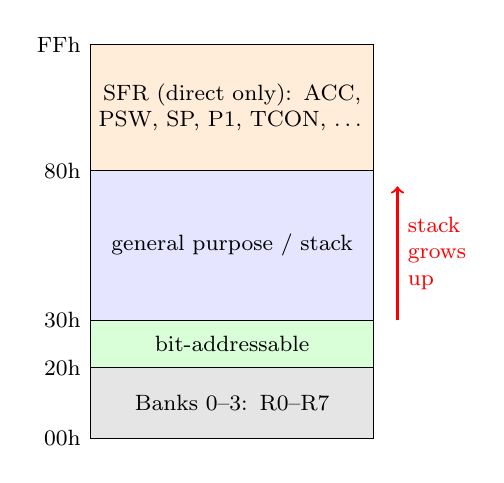
\begin{tikzpicture}[x=1cm,y=1cm,font=\footnotesize]
      \foreach \y/\h/\c/\t/\a in {0/0.9/gray!20/{Banks 0--3: R0--R7}/00h,
                                  0.9/0.6/green!15/{bit-addressable}/20h,
                                  1.5/1.9/blue!10/{general purpose / stack}/30h,
                                  3.4/1.6/orange!15/{SFR (direct only): ACC, PSW, SP, P1, TCON, \dots}/80h}{
        \draw[fill=\c] (0,\y) rectangle (3.6,\y+\h);
        \node[align=center,text width=3.4cm] at (1.8,\y+\h/2) {\t};
        \node[left] at (0,\y) {\a};
      }
      \node[left] at (0,5) {FFh};
      \draw[->,thick,red] (3.9,1.5) -- (3.9,3.2) node[midway,right,align=left]{stack\\grows\\up};
    \end{tikzpicture}
    \end{column}
    \begin{column}{0.53\textwidth}
      \begin{itemize}
        \item PSW bits RS1, RS0 select the active register bank: a fast context switch for ISRs.
        \item Reset: SP = 07h, the first PUSH writes 08h, which is register bank~1. Set SP before using bank~1 or variables.
        \item \texttt{PUSH}: SP $\leftarrow$ SP+1, then write. \texttt{POP}: read, then SP $\leftarrow$ SP$-$1.
        \item Only 128 bytes of RAM for registers, variables, \emph{and} stack.
      \end{itemize}
    \end{column}
  \end{columns}
\end{frame}

\subsection{Fetch, decode, execute}
\begin{frame}{The instruction cycle}
  \begin{center}
  \begin{tikzpicture}[>=Stealth,font=\footnotesize,
      st/.style={draw,rounded corners,fill=blue!10,minimum width=3.0cm,minimum height=0.8cm,align=center}]
    \node[st] (f) at (0,0)    {\textbf{Fetch}\\MAR $\leftarrow$ PC, IR $\leftarrow$ M[MAR]\\PC $\leftarrow$ PC+1};
    \node[st] (d) at (4.8,0)  {\textbf{Decode}\\operation, addressing mode,\\operand bytes (PC+1 each)};
    \node[st] (e) at (4.8,-2) {\textbf{Execute}\\ALU / transfer, write result,\\flags, or new PC};
    \node[st,fill=red!10] (i) at (0,-2) {\textbf{Interrupt check}\\pending and enabled?};
    \node[st,fill=red!10] (v) at (-4.4,-2) {push PC\\PC $\leftarrow$ vector};
    \draw[->,thick] (f) -- (d);
    \draw[->,thick] (d) -- (e);
    \draw[->,thick] (e) -- (i);
    \draw[->,thick] (i) -- node[left]{no} (f);
    \draw[->,thick] (i) -- node[above]{yes} (v);
    \draw[->,thick] (v) |- (f);
  \end{tikzpicture}
  \end{center}
  \begin{itemize}
    \item The cycle never stops: after reset PC = 0000h, the reset vector.
    \item Interrupts are only accepted \emph{between} instructions.
  \end{itemize}
\end{frame}

\scriptonly{%
\textbf{Fetch.} The PC is copied to the MAR and put on the address bus; the byte read from program memory is the opcode and goes into the IR. The PC is incremented and now points to the next byte.

\textbf{Decode.} The control unit decodes the opcode: which operation, which addressing mode (immediate, direct, register, indirect), and how many operand bytes follow. The operand bytes are fetched in the same way, each one incrementing the PC. When decoding is complete, the PC already points to the next instruction.

\textbf{Execute.} The control unit drives the ALU and the data paths: the result is written to a register or memory, the flags in the PSW are updated, or, for jumps and calls, a new value is loaded into the PC.

\textbf{Interrupt check.} At the end of each instruction the CPU checks for pending and enabled interrupts. If one is accepted, the hardware executes a call to the interrupt vector instead of fetching the next instruction. A long instruction therefore delays the reaction to an interrupt; this is part of the latency $T_L$.
}

\begin{frame}{Example: tracing four instructions}
  \footnotesize
  \begin{tabular}{@{}llllllll@{}}
    \toprule
    PC & bytes & instruction & execute & A & CY & PC after & cycles \\
    \midrule
    0030h & 74 05 & \texttt{MOV A,\#05h}  & A $\leftarrow$ 05h & 05h & 0 & 0032h & 1 \\
    0032h & 24 FD & \texttt{ADD A,\#0FDh} & A $\leftarrow$ A + FDh & 02h & 1 & 0034h & 1 \\
    0034h & F5 90 & \texttt{MOV P1,A}     & P1 $\leftarrow$ A & 02h & 1 & 0036h & 1 \\
    0036h & 80 F8 & \texttt{SJMP 0030h}   & PC $\leftarrow$ 0038h + (F8h = $-8$) & 02h & 1 & 0030h & 2 \\
    \bottomrule
  \end{tabular}
  \medskip
  \begin{itemize}
    \item The opcode (74h, 24h, F5h, 80h) tells the decoder how many operand bytes follow.
    \item \texttt{ADD} sets the flags: CY = 1 (05h + FDh = 102h), AC = 1, OV = 0 ($5 + (-3) = 2$), P = 1 (odd number of ones in A).
    \item Relative jumps are computed from the PC \emph{after} the fetch.
    \item One loop: $1+1+1+2 = 5$ machine cycles.
  \end{itemize}
\end{frame}

\scriptonly{%
Exercise: run these four instructions in EdSim51 with the Step button and watch PC, A, and PSW. Then encode \texttt{MOV A,\#3Fh} and \texttt{ADD A,\#0C1h} yourself (8051 instruction set table) and predict all four flags.
}

\begin{frame}{Machine cycles and time}
  \begin{itemize}
    \item 8051: one \emph{machine cycle} = 12 oscillator periods (6 states with 2 phases each). At 12\,MHz (EdSim51 default): 1\,machine cycle = 1\,\textmu s.
    \item Instructions take 1, 2, or 4 machine cycles (\texttt{MUL}, \texttt{DIV}). The number is fixed per instruction and listed in the data sheet.
    \item AVR (Arduino Uno): two-stage pipeline, the next instruction is fetched while the current one executes $\Rightarrow$ most instructions take 1 clock (62.5\,ns at 16\,MHz), branches and calls 2--4.
    \item No cache, no branch prediction: the execution time of a path is the \emph{sum} of the cycle counts. This is what makes static analysis on small microcontrollers practical.
  \end{itemize}
\end{frame}

\subsection{Calls and interrupts}
\begin{frame}{Subroutines and the stack}
  \begin{columns}[T]
    \begin{column}{0.5\textwidth}
      \texttt{CALL work} at 007Bh in example~6 (3 bytes):
      \begin{enumerate}
        \item return address $= 007\text{Eh}$
        \item SP+1, M[SP] $\leftarrow$ 7Eh (low byte)
        \item SP+1, M[SP] $\leftarrow$ 00h (high byte)
        \item PC $\leftarrow$ address of \texttt{work}
      \end{enumerate}
      \texttt{RET}: PC high $\leftarrow$ M[SP], SP$-$1, PC low $\leftarrow$ M[SP], SP$-$1.
    \end{column}
    \begin{column}{0.48\textwidth}
      \begin{itemize}
        \item The stack is the only place where the CPU remembers \emph{where to continue}.
        \item Last in, first out: the most recent call returns first.
        \item \texttt{PUSH}/\texttt{POP} store registers on the same stack.
        \item Nothing checks the SP against a limit.
      \end{itemize}
    \end{column}
  \end{columns}
\end{frame}

\begin{frame}{Interrupts on the 8051}
  \begin{itemize}
    \item An interrupt is a \emph{call generated by hardware}: push PC (2 bytes), PC $\leftarrow$ vector: 0003h INT0, 000Bh Timer~0, 0013h INT1, 001Bh Timer~1, 0023h serial.
    \item Only the PC is saved. ACC, PSW, and registers must be saved by the ISR (\texttt{PUSH} or bank switch).
    \item An internal ``interrupt in progress'' flag blocks further interrupts of the same priority level until \texttt{RETI}. \texttt{RET} does \emph{not} clear it.
    \item Each source has \emph{one} pending flag (e.g.\ TF0). A second event while the flag is set is lost.
    \item After \texttt{RETI} at least one instruction of the interrupted program is executed.
    \item Response time: 3 to 9 machine cycles from flag to first ISR instruction.
  \end{itemize}
\end{frame}

\scriptonly{%
The AVR behaves in the same way with different names: the hardware pushes the PC and clears the I flag in SREG, so no other interrupt is accepted; \texttt{reti} sets the I flag again. SREG and the registers are saved by code that the compiler generates. Each interrupt source has one flag, and a second event while it is set is lost.
}

% ===========================================================================
\section{Interrupt Experiments in EdSim51}
\label{sec:edsim}

\begin{frame}{EdSim51: an 8051 simulator}
  \begin{itemize}
    \item Java program, free download: \url{https://www.edsim51.com/}
    \item Shows PC, SP, ACC, PSW, internal RAM, and all SFRs, while running or in single steps.
    \item Peripherals: LEDs on P1 (active low), switches on P2, 7-segment display, keypad, ADC/DAC, UART.
    \item Workflow: \emph{Load} the \texttt{.asm} file, \emph{Assm}, then \emph{Step} or \emph{Run}. Clock: 12\,MHz $\Rightarrow$ 1\,\textmu s per machine cycle.
    \item Examples: \texttt{examples/ex05\_8051\_isr\_overrun}, \texttt{examples/ex06\_8051\_stack\_overflow}
  \end{itemize}
\end{frame}

\scriptonly{%
The examples in this chapter are plain 8051 assembler and are not Wokwi projects: the effects are visible at the level of single instructions, stack bytes, and machine cycles, which EdSim51 shows directly. The Arduino Uno behaves the same way in principle (see the comparison table above). Both examples were checked with a cycle-accurate model of the instructions they use; the cycle numbers given below are computed from the 8051 instruction set and should be confirmed in EdSim51.
}

\begin{frame}{Is something wrong? Decide before you run}
  \begin{itemize}
    \item The errors in examples 5 and 6 are \alert{silent}: no crash, no message, the program keeps running. The symptoms appear late and far away from the cause.
    \item Therefore write down first what a correct run must show, then compare:
  \end{itemize}
  \begin{center}\footnotesize
  \begin{tabular}{@{}lll@{}}
    \toprule
    Invariant & Watch & Broken by \\
    \midrule
    ISR runs = elapsed time$/T$ & TICKS vs.\ time & lost ticks (ex.~5) \\
    no overflow pending at ISR end & OVERRUN = 0 & $C > T$ (ex.~5) \\
    background makes progress & main counter, LEDs & starvation (ex.~5) \\
    SP returns to its base value & SP & nesting (ex.~6) \\
    nesting depth $\le 1$ & DEPTH, MAXDEPTH & nesting (ex.~6) \\
    data next to the stack unchanged & SETPOINT, output & stack overflow (ex.~6) \\
    \bottomrule
  \end{tabular}
  \end{center}
\end{frame}

\scriptonly{%
Both examples contain a design error that the hardware does not report. The 8051 has no counter for lost interrupt requests and no stack limit; the program simply continues with wrong timing or corrupted data. Whoever runs the examples without a clear expectation will see blinking LEDs and changing numbers and conclude that everything works. The table lists the invariants of a correct interrupt-driven system and the variables in the examples that make them observable. Each example file starts with a block ``How to spot the error'' that lists, for both switch positions, what to look at and when the first symptom appears.
}

\subsection{ISR longer than its period}
\begin{frame}[fragile]{Example 5: ISR with long work}
  \begin{columns}[T]
    \begin{column}{0.62\textwidth}
\lstinputlisting[style=asm51,basicstyle=\ttfamily\fontsize{6}{7}\selectfont,linerange={75-92},numbers=none]{examples/ex05_8051_isr_overrun/isr_overrun.asm}
    \end{column}
    \begin{column}{0.36\textwidth}
      \small
      \begin{itemize}
        \item Timer~0, mode 2: tick every $T = 200$\,\textmu s.
        \item SW0 selects the work: $N = 40$ or $N = 230$ loop passes.
        \item TICKS counts ISR runs, OVERRUN counts ISRs that end with TF0 already set again.
        \item Main loop: 16-bit counter, high byte on the LEDs.
      \end{itemize}
    \end{column}
  \end{columns}
\end{frame}

\scriptonly{%
\edsimexample{ex05_8051_isr_overrun}{isr_overrun}{EdSim51 example 5: ISR work longer than the interrupt period}{lst:ex05}

Example~\ref{lst:ex05} sets the stack pointer to 2Fh first, because the ISR uses register bank~1 (08h--0Fh), exactly where the stack would start after reset. Timer~0 runs in mode~2: TL0 counts machine cycles and is reloaded from TH0 on overflow, so with a reload value of $256-200 = 56$ the overflow flag TF0 is set every 200 machine cycles. The ISR saves PSW and ACC, switches to register bank~1 and calls \texttt{work}, a busy loop of $2N + 2$ cycles. The right-hand comment column of the file lists the machine cycles of each instruction.
}

\begin{frame}{Example 5: what happens with long work}
  \begin{center}
  \begin{tikzpicture}[x=1.05cm,y=1cm,>=Stealth,font=\footnotesize]
    \draw[->] (0,0) -- (10.6,0) node[right]{$t$ [\textmu s]};
    \foreach \t/\s in {0/ok,2/pend,4/lost,6/pend,8/lost,10/pend}{
      \draw (\t,-0.1) -- (\t,0.1);
      \node[below] at (\t,-0.1) {\pgfmathparse{int(\t*100)}\pgfmathresult};
    }
    \foreach \t in {0,2,6,10}{\draw[->,thick,blue] (\t,1.6) -- (\t,1.15);}
    \foreach \t in {4,8}{\node[red,font=\bfseries] at (\t,1.4) {$\times$};}
    \node[left,blue] at (-0.1,1.4) {TF0};
    \draw[fill=red!25] (0,0.2) rectangle (4.88,0.8) node[midway]{ISR 1: 488 cycles};
    \draw[fill=red!25] (4.9,0.2) rectangle (9.78,0.8) node[midway]{ISR 2};
    \draw[fill=red!25] (9.8,0.2) rectangle (10.5,0.8);
    \draw[fill=green!40] (4.88,0.2) rectangle (4.9,0.8);
    \draw[fill=green!40] (9.78,0.2) rectangle (9.8,0.8);
    \node[green!40!black,align=center] at (4.89,-0.85) {1 instruction of main};
    \draw[->,green!40!black] (4.89,-0.65) -- (4.89,0.15);
  \end{tikzpicture}
  \end{center}
  \begin{itemize}
    \item TF0 is set at 200\,\textmu s while ISR~1 runs (pending), at 400\,\textmu s it is still set: this tick is \textcolor{red}{lost}.
    \item After 20\,ms: 99 timer overflows, but only 41 ISR runs (TICKS), 40 of them with OVERRUN. MAINHI stays 0.
    \item With $N = 40$: ISR 106\,\textmu s, TICKS = 99, OVERRUN = 0, main gets about half the CPU (MAINHI = 9).
  \end{itemize}
\end{frame}

\scriptonly{%
The ISR needs 488 machine cycles, almost 2.5 periods. Hardware remembers only one pending overflow per source, so of the 2.44 overflows per ISR run, 1.44 are lost: the system silently runs at a lower rate than the one programmed. Between two ISR runs the CPU returns to the main program for exactly one instruction, because the 8051 always executes one instruction after \texttt{RETI} before it accepts the next interrupt. The main loop therefore advances by one instruction every 489\,\textmu s and appears frozen. Nothing in the hardware reports the problem; only the software check of TF0 at the end of the ISR makes it visible.
}

\begin{frame}{Example 5: how to spot the error in EdSim51}
  \begin{center}\footnotesize
  \begin{tabular}{@{}lll@{}}
    \toprule
    Watch & SW0 = 1 (short, correct) & SW0 = 0 (long, wrong) \\
    \midrule
    TICKS (20h) after 20\,ms & 63h (99): one per 200\,\textmu s & 29h (41): one per 489\,\textmu s \\
    OVERRUN (21h) & stays 0 & +1 after \emph{every} ISR: 28h (40) \\
    LEDs (MAINHI) & count up & never change \\
    TF0 in the SFR panel & 0 when the ISR ends & already 1 when the ISR ends \\
    \bottomrule
  \end{tabular}
  \end{center}
  \begin{itemize}
    \item \textbf{When:} the first ISR is still running when TF0 is set again (pending), and once more 200\,\textmu s later: lost. The first ISR ends after 488\,\textmu s with TF0 = 1, OVERRUN becomes 1.
    \item \textbf{Where to look:} single-step over \texttt{JNB TF0,isrEnd}, the program's only error check. Without it, only the LEDs show that something is wrong, and only if you know they should count.
  \end{itemize}
\end{frame}

\subsection{Resuming later: nested interrupts}
\begin{frame}[fragile]{Example 6: let the next tick preempt the work?}
  \begin{columns}[T]
    \begin{column}{0.62\textwidth}
\lstinputlisting[style=asm51,basicstyle=\ttfamily\fontsize{6}{7}\selectfont,linerange={70-72,85-101},numbers=none]{examples/ex06_8051_stack_overflow/stack_overflow.asm}
    \end{column}
    \begin{column}{0.36\textwidth}
      \small
      \begin{itemize}
        \item Idea: the next tick should interrupt the running work, and the old work should \emph{resume where it left off} afterwards.
        \item The 8051 blocks the same level until \texttt{RETI}. Trick: \texttt{CALL} a \texttt{RETI}.
        \item Same as \texttt{sei()} in an AVR ISR or \texttt{ISR\_NOBLOCK} in avr-libc.
        \item Each level: PC, ACC, PSW, R7, return address $= 7$ bytes.
      \end{itemize}
    \end{column}
  \end{columns}
\end{frame}

\scriptonly{%
\edsimexample{ex06_8051_stack_overflow}{stack_overflow}{EdSim51 example 6: nested interrupts lead to a stack overflow}{lst:ex06}

In Example~\ref{lst:ex06} the ISR calls \texttt{allowNesting}, which consists of a single \texttt{RETI}. This pops the return address, as \texttt{RET} would, and additionally clears the ``interrupt in progress'' flag. From then on the ISR runs like normal code, and the next Timer~0 overflow interrupts it. The ISR therefore ends with \texttt{RET}. Each ISR instance outputs the variable SETPOINT (60h) to the LEDs, as a controller would output its setpoint to an actuator, and the ISR checks at its entry whether SP has reached the limit 78h.
}

\begin{frame}{Example 6: the stack with long work}
  \begin{columns}[T]
    \begin{column}{0.45\textwidth}
    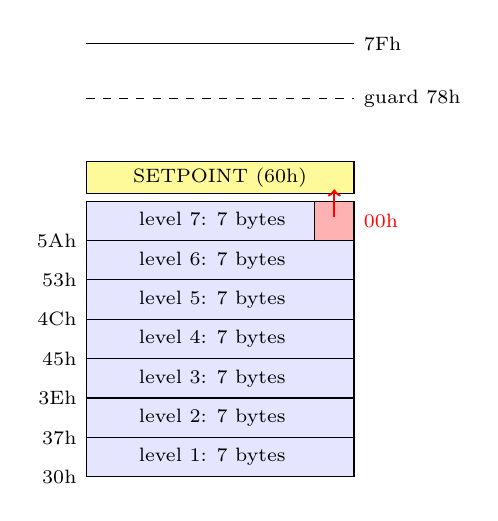
\begin{tikzpicture}[x=1cm,y=0.5cm,font=\scriptsize]
      \foreach \k in {1,...,7}{
        \pgfmathtruncatemacro{\a}{48+7*(\k-1)}
        \draw[fill=blue!10] (0,\k-1) rectangle (3.4,\k);
        \node at (1.6,\k-0.5) {level \k: 7 bytes};
        \node[left] at (0,\k-1) {\pgfmathparse{Hex(\a)}\pgfmathresult h};
      }
      \draw[fill=red!30] (2.9,6) rectangle (3.4,7);
      \draw[fill=yellow!40] (0,7.2) rectangle (3.4,8) node[midway]{SETPOINT (60h)};
      \draw[->,red,thick] (3.15,6.6) -- (3.15,7.3);
      \node[red,right] at (3.4,6.5) {00h};
      \draw[dashed] (0,9.6) -- (3.4,9.6) node[right]{guard 78h};
      \draw (0,11) -- (3.4,11) node[right]{7Fh};
      \node[left] at (0,0) {};
    \end{tikzpicture}
    \end{column}
    \begin{column}{0.53\textwidth}
      \begin{itemize}
        \item SW0 = short: every ISR ends before the next tick, MAXDEPTH = 1, SP $\le$ 36h.
        \item SW0 = long: every tick adds a level. At depth~7 (1.4\,ms) the return address of level~7 overwrites SETPOINT: the LEDs go dark.
        \item At depth~11 (2.2\,ms) the guard stops the program: all LEDs on.
        \item Without the guard (classic 8051, 128 bytes RAM): bytes pushed beyond 7Fh are lost, SP wraps to 00h and overwrites R0--R7.
      \end{itemize}
    \end{column}
  \end{columns}
\end{frame}

\begin{frame}{Example 6: how to spot the error in EdSim51}
  \begin{center}\footnotesize
  \begin{tabular}{@{}lll@{}}
    \toprule
    Watch & SW0 = 1 (short, correct) & SW0 = 0 (long, wrong) \\
    \midrule
    SP & stays $\le$ 36h & +7 every 200\,\textmu s, never comes back \\
    DEPTH / MAXDEPTH & 1 / 1 & +1 every period \\
    RAM 30h..7Fh & same few bytes change & filled level by level \\
    LEDs (SETPOINT) & 4..7 on & 4..7 on, then dark, then all on \\
    \bottomrule
  \end{tabular}
  \end{center}
  \begin{itemize}
    \item \textbf{2nd tick:} DEPTH = 2. This alone is the error: with $C > T$ the depth can only grow.
    \item \textbf{Depth 7 (1.4\,ms):} a return address overwrites SETPOINT (60h). Nothing reports it, the ISR outputs garbage: the LEDs go dark.
    \item \textbf{Depth 11 (2.2\,ms):} SP $\ge$ 78h, the guard stops the program, all LEDs on. Without the guard: wrong output first, crash later, if at all.
  \end{itemize}
\end{frame}

\begin{frame}{Why ``resume later'' cannot work}
  \begin{itemize}
    \item Nested interrupts use one stack: \emph{last in, first out}. Level~1 can only resume after levels 2, 3, \dots\ have finished.
    \item With $C > T$ a new level always arrives first: the oldest work never resumes, the depth grows by one per period:
    \[ d(t) = \left\lfloor t/T \right\rfloor + 1, \qquad \text{stack}(t) = 7\,d(t)\ \text{bytes} \]
    \item Without nesting (example 5) ticks are lost, with nesting (example 6) the stack overflows. Both violate the load condition $\rho = C/T < 1$.
    \item Resuming a job ``where it left off'' needs its own context, i.e.\ its own stack: a \emph{task}. An RTOS gives every task a stack and lets the scheduler decide what resumes (from Chapter~\ref{sec:tasks} on).
    \item ISRs must stay short: acknowledge, read data, signal a task (\texttt{xSemaphoreGiveFromISR}).
  \end{itemize}
\end{frame}

\scriptonly{%
A task does not remove the load problem: if a periodic job needs more processor time than its period, no scheduler can meet all deadlines. But a task-based design makes the problem visible and controllable. A missed deadline can be counted (Example~4 in Chapter~\ref{sec:runtimestats} will show how), lower-priority work is delayed in a defined way, and the stack of each task has a fixed, known size, independent of how often the event occurs.
}

\begin{frame}{Stack overflow: causes, effects, detection}
  \begin{description}
    \item[Causes] recursion, nested interrupts, large local variables, deep call chains, stack placed too close to data (SP = 07h after reset).
    \item[Effects] silent corruption of variables and registers; overwritten return addresses send the PC to random code. Often far away from the cause, and only under load.
    \item[Detection at run time] SP limit check (example 6), fill pattern (\emph{watermark}) or canary at the stack end; FreeRTOS: \texttt{configCHECK\_FOR\_STACK\_OVERFLOW} and \texttt{uxTaskGetStackHighWaterMark()}.
    \item[Prevention] static stack analysis (next section).
  \end{description}
\end{frame}

\subsection{Without installation: the web simulator}
\begin{frame}[fragile]{Examples 5 and 6 in the browser}
  \begin{columns}[T]
    \begin{column}{0.55\textwidth}
\lstinputlisting[style=asm51,basicstyle=\ttfamily\fontsize{6}{7}\selectfont,linerange={116-130},numbers=none]{examples/ex05_8051_isr_overrun/isr_overrun_sim8.asm}
    \end{column}
    \begin{column}{0.43\textwidth}
      \small
      \begin{itemize}
        \item \url{https://schweigi.github.io/assembler-simulator/}: 8-bit CPU, registers A--D, 256 bytes RAM, console at E8h--FFh, stack from E7h downwards.
        \item No timer, no interrupts: subroutine \texttt{tick} emulates both, once per loop pass. Time = number of \texttt{tick} calls, period 10.
        \item \texttt{INPROG} plays the 8051 ``interrupt in progress'' flag, \texttt{reti} clears it.
        \item Files \texttt{*\_sim8.asm}; work length: \texttt{NWORK} = 4 or 25.
      \end{itemize}
    \end{column}
  \end{columns}
\end{frame}

\scriptonly{%
EdSim51 must be installed (Java). The browser-based simulator by Schweigi needs no installation, but it simulates a much simpler CPU: four general-purpose registers, a stack pointer, the flags Z and C, 256 bytes of memory shared by code, data and stack, and a 24-character console mapped to E8h--FFh. It has neither a timer nor interrupts nor input pins. The files \texttt{isr\_overrun\_sim8.asm} and \texttt{stack\_overflow\_sim8.asm} in the folders of examples~5 and~6 therefore emulate the hardware in software: the subroutine \texttt{tick} is one clock of a timer with period~10. On overflow it sets TF, and if TF is set and no ISR is in progress (\texttt{INPROG} = 0), it clears TF, sets \texttt{INPROG} and jumps to the ISR, which returns to the caller of \texttt{tick}. The routine \texttt{reti} clears \texttt{INPROG} and returns, exactly the part of \texttt{RETI} the experiments depend on. Because every loop calls \texttt{tick} once per pass, interrupts are only accepted at these points, and time is counted in \texttt{tick} calls rather than machine cycles. The switch SW0 is replaced by the variable \texttt{NWORK} at address 08h, which is edited in the source before assembling.

\lstinputlisting[style=asm51,caption={Web simulator version of example 5},label={lst:ex05web}]{examples/ex05_8051_isr_overrun/isr_overrun_sim8.asm}

In Example~\ref{lst:ex05web} the console shows a timeline with one character per tick: \texttt{.} for the main loop, \texttt{\#} for the ISR, \texttt{|} for a timer overflow and \texttt{X} for an overflow while TF was still set, i.e.\ a lost tick. With $\mathtt{NWORK} = 4$ the pattern \texttt{|\#\#\#\#.....} repeats and TICKS (02h) equals PERIODS (03h). With $\mathtt{NWORK} = 25$ the ISR runs for 2.5 periods: after 13 periods only 5 ISRs have run, OVERRUN (04h) counts every ISR, and only one main loop pass (\texttt{.}) fits between two ISRs, the counterpart of the one instruction on the 8051.

\lstinputlisting[style=asm51,caption={Web simulator version of example 6},label={lst:ex06web}]{examples/ex06_8051_stack_overflow/stack_overflow_sim8.asm}

Example~\ref{lst:ex06web} calls \texttt{reti} early, as \texttt{allowNesting} does on the 8051. Each nesting level puts 4 bytes on the stack: the return address of the interrupted \texttt{tick} call, A, B and the return address of \texttt{work}. The memory view marks the stack area, which grows downwards from E7h by 4 bytes per period. The console shows SETPOINT as a character and one \texttt{>} per nesting level. With long work, the stack overwrites SETPOINT at depth~18 with a byte of a return address. Nothing happens at that moment; only the ISR at depth~19 outputs the corrupted value, and the \texttt{S} on the console turns into a \texttt{C}. When level~21 starts, the guard \texttt{CMP SP, LIMIT} stops the CPU with \texttt{!}. Without the guard the stack would run into the code, as there is no separation between code, data, and stack in this memory.
}

\begin{frame}[fragile]{Example 5 in the browser: reading the timeline}
  \footnotesize
  Console after 40 ticks (one character per tick, starting at tick 1):
\begin{verbatim}
NWORK = 4 : .........|####.....|####.....|####.....|
NWORK = 25: .........|#########|#########X#####.###|
tick:               10        20        30
\end{verbatim}
  \begin{itemize}
    \item \textbf{Tick 20:} \texttt{|} inside the \texttt{\#} block: the next overflow arrives while the ISR still runs (pending, not yet lost).
    \item \textbf{Tick 30:} \texttt{X}: TF is still set, this tick is lost. Real hardware shows nothing here.
    \item \textbf{Afterwards:} one \texttt{.} between ISRs, then the next ISR starts without a \texttt{|}: it serves an old, delayed tick.
    \item \textbf{Counters (memory view):} TICKS (02h) falls behind PERIODS (03h), e.g.\ 5 ISRs in 13 periods; OVERRUN (04h) +1 per ISR; MAINCNT (05h) +1 per ISR instead of +6 per period.
    \item The timeline wraps after 24 ticks: \emph{Stop} or \emph{Step} to read it.
  \end{itemize}
\end{frame}

\begin{frame}{Example 6 in the browser: watching the stack}
  \begin{columns}[T]
    \begin{column}{0.40\textwidth}
    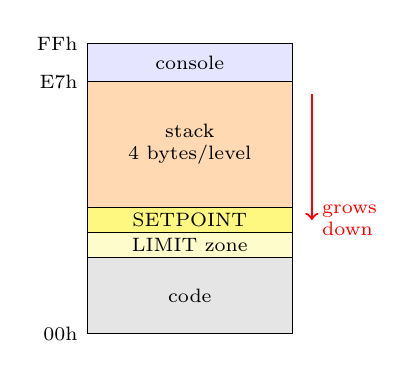
\begin{tikzpicture}[x=1cm,y=0.32cm,font=\scriptsize]
      \draw[fill=gray!20] (0,0) rectangle (2.6,3) node[midway]{code};
      \draw[fill=yellow!20] (0,3) rectangle (2.6,4) node[midway]{LIMIT zone};
      \draw[fill=yellow!50] (0,4) rectangle (2.6,5) node[midway]{SETPOINT};
      \draw[fill=orange!30] (0,5) rectangle (2.6,10) node[midway,align=center]{stack\\4 bytes/level};
      \draw[fill=blue!10] (0,10) rectangle (2.6,11.5) node[midway]{console};
      \node[left] at (0,10) {E7h};
      \node[left] at (0,11.5) {FFh};
      \node[left] at (0,0) {00h};
      \draw[->,red,thick] (2.85,9.5) -- (2.85,4.5) node[right,align=left]{grows\\down};
    \end{tikzpicture}
    \end{column}
    \begin{column}{0.58\textwidth}
      \small
      \begin{itemize}
        \item \textbf{Correct (NWORK = 4):} SP between E1h and E7h, DEPTH 0/1, one \texttt{>}, console \texttt{S}.
        \item \textbf{Period 2:} DEPTH = 2, SP does not return. This is already the error.
        \item \textbf{Depth 18:} the stack reaches SETPOINT. Silent.
        \item \textbf{Depth 19:} the ISR outputs the corrupted value: \texttt{S} $\to$ \texttt{C}.
        \item \textbf{Level 21:} SP $<$ LIMIT, guard stops the CPU: \texttt{!}.
        \item Same memory for code, data, stack: without the guard the stack overwrites \texttt{reti} next.
      \end{itemize}
    \end{column}
  \end{columns}
\end{frame}

\scriptonly{%
In the browser versions the first symptom is always visible long before the visible failure. In example~5 the first \texttt{X} appears at tick~30, during the first ISR; from then on the counters TICKS and PERIODS drift apart. In example~6 the depth of 2 in the second period already proves the error, because with work longer than the period the depth can only grow. The corrupted output appears 17 periods later, the stop only after 20 periods. A test that only looks for a crash or a wrong output would need to run that long, and on a real controller with more RAM much longer; checking the invariants finds the error in the first periods.
}

% ===========================================================================
\section{Nested Interrupts on the AVR: Watching the Stack in the Debugger}
\label{sec:avrnesting}

\begin{frame}[fragile]{Example 8: example 6 in Arduino C}
  \begin{columns}[T]
    \begin{column}{0.60\textwidth}
\lstinputlisting[basicstyle=\ttfamily\fontsize{6}{7}\selectfont,linerange={82-104},numbers=none]{examples/ex08_avr_isr_nesting/sketch.ino}
    \end{column}
    \begin{column}{0.38\textwidth}
      \small
      \begin{itemize}
        \item Timer~1 every $T = 1$\,ms, work 0.3\,ms or 2.5\,ms (DIP switch~1).
        \item The AVR clears I on ISR entry; \texttt{sei()} sets it again: the \texttt{allowNesting} of example~6.
        \item Stack from \texttt{RAMEND} (8FFh) \emph{downwards}, towards the static variables. \texttt{app} lies in \texttt{.noinit}, right after \texttt{.bss}: the first data the stack meets.
        \item 22 bytes per level: 18 pushed registers, return address, call of \texttt{work}.
      \end{itemize}
    \end{column}
  \end{columns}
\end{frame}

\scriptonly{%
\wokwiexample{ex08_avr_isr_nesting}{Nested timer interrupts on the AVR without an RTOS}{lst:ex08}

Example~\ref{lst:ex08} transfers example~6 to the ATmega328P of the Arduino Uno. The AVR has no ``interrupt in progress'' flag per level; instead it clears the global interrupt flag I in SREG when it enters an ISR, and \texttt{RETI} sets it again. An ISR that executes \texttt{sei()} can therefore be interrupted by any interrupt, including its own. avr-libc offers the same as \texttt{ISR\_NOBLOCK}, which places the \texttt{sei} before the prologue. The example executes \texttt{sei()} only after its bookkeeping, so that \texttt{depth}, \texttt{maxDepth} and \texttt{levelSP[]} are updated atomically.

The stack of the AVR grows from \texttt{RAMEND} (8FFh) downwards. Below it lie the free RAM, the heap (unused here), and the static variables in the order \texttt{.data}, \texttt{.bss}, \texttt{.noinit}. Placing \texttt{app} in \texttt{.noinit} makes it the variable with the highest address, so the stack meets \texttt{app.setpoint} first, just as it met SETPOINT on the 8051. The guard \texttt{STACK\_LIMIT} leaves room for one more ISR frame below \texttt{app}; a guard that only trips once SP lies below the protected data would let the frame that trips it overwrite the variables below.

The empty functions \texttt{dbgNested}, \texttt{dbgSetpointCorrupted} and \texttt{dbgStackOverflow} do nothing at run time. They mark the moments worth looking at, and the debugger sets its breakpoints on them.
}

\begin{frame}{Debugging with Wokwi for VS Code}
  \begin{itemize}
    \item Wokwi simulates the firmware built by PlatformIO and offers a GDB server (port 3333). VS Code connects \texttt{avr-gdb} to it (\texttt{.vscode/launch.json}).
    \item \texttt{debug.gdb} (loaded automatically) sets the breakpoints and defines views for the Debug Console: \texttt{-exec levels}, \texttt{-exec sv}, \texttt{-exec memmap}.
    \item A breakpoint stops the whole simulated CPU, timers included: after \emph{Continue} the program runs on as if there had been no pause.
  \end{itemize}
  \begin{center}\footnotesize
  \begin{tabular}{@{}lll@{}}
    \toprule
    Breakpoint & long work & what to look at \\
    \midrule
    \texttt{dbgNested} & 2\,ms, depth 2 & SP of both levels, SREG.I = 0 \\
    \texttt{dbgSetpointCorrupted} & 79\,ms, level 79 & \texttt{app.setpoint} = 4Eh, SP $<$ \&\texttt{app.setpoint} \\
    \texttt{dbgStackOverflow} & 83\,ms, level 83 & guard: SP $<$ \texttt{STACK\_LIMIT} \\
    \bottomrule
  \end{tabular}
  \end{center}
  \begin{itemize}
    \item Sidebar: \emph{Registers $\to$ CPU} (r0--r31, SREG, SP, PC), \emph{Watch}: \texttt{depth}, \texttt{levelSP}, \texttt{app}.
  \end{itemize}
\end{frame}

\begin{frame}[fragile]{Example 8 in the debugger: one frame per tick}
\begin{verbatim}
Breakpoint 3, dbgSetpointCorrupted (level=79, value=78 'N')
0x8ff  RAMEND, the stack starts here and grows down
0x233  SP (stack used: 1740 bytes)
       free: -5 bytes (negative: the stack has passed app.setpoint)
0x238  app.setpoint = 0x4e (0xf0 = intact)
0x1f0  STACK_LIMIT, guard trips when SP is below
level   SP    bytes  interrupted code (return address on the stack)
    1  0x8e9    -   main + 12 in section .text
    2  0x8d3   22   work(unsigned char) + 8 in section .text
  ...
   79  0x235   22   work(unsigned char) + 10 in section .text
\end{verbatim}
  \begin{itemize}
    \small
    \item Every level from 2 on has interrupted \texttt{work()} of the level before: none of them will ever resume.
    \item Level 79 has pushed its own registers over \texttt{app.setpoint}; the same ISR outputs the wrong value.
    \item $\text{stack}(t) = 22\,d(t)$ bytes: the formula of example~6 with 22 instead of 7.
  \end{itemize}
\end{frame}

\scriptonly{%
The command \texttt{levels} reads \texttt{levelSP[]}, the stack pointer each level stored right after its prologue, and finds the return address above the 18 pushed registers. The hardware pushes the program counter as a word address, high byte at the lower address; multiplied by two it is a byte address that GDB translates into a function and an offset. The output shows the mechanism of example~6 directly: level~1 interrupted the empty main loop, every further level interrupted the busy loop in \texttt{work()} of the level before, and the distance between two levels is always 22 bytes. GDB writes RAM addresses with an offset of 800000h (e.g.\ \texttt{0x8008d2}), because on the AVR flash and RAM both start at address~0.

With the short work the depth stays~1 and none of the three breakpoints is hit. To look at a single ISR in that case, enable the breakpoint on \texttt{dbgTick}, which is called at every ISR entry: \texttt{-exec info breakpoints} lists the numbers, \texttt{-exec enable} $n$ enables it.
}

\begin{frame}[fragile]{Example 9: the same ISR under FreeRTOS}
  \begin{columns}[T]
    \begin{column}{0.55\textwidth}
\lstinputlisting[basicstyle=\ttfamily\fontsize{6}{7}\selectfont,linerange={106-106,121-134},numbers=none]{examples/ex09_rtos_isr_nesting/sketch.ino}
    \end{column}
    \begin{column}{0.43\textwidth}
      \small
      \begin{itemize}
        \item An AVR ISR has no stack of its own: it pushes onto the stack of the \emph{interrupted task}.
        \item Task stacks are blocks of fixed size on the FreeRTOS heap; below each one lies the previous block.
        \item DIP switch~2: work in the ISR (nesting) or in a Worker task, the ISR only notifies (\emph{deferred interrupt handling}).
      \end{itemize}
    \end{column}
  \end{columns}
\end{frame}

\scriptonly{%
\wokwiexample{ex09_rtos_isr_nesting}{The nested ISR of example 8 under FreeRTOS}{lst:ex09}

Example~\ref{lst:ex09} uses the ISR of example~8 in a FreeRTOS application (tasks are introduced in Chapter~\ref{sec:tasks}). The Ctrl task outputs the setpoint every tick and otherwise waits, so the Idle task runs most of the time and is the task the timer interrupt usually interrupts. The Ctrl task also reads the DIP switches right after each tick, so that a phase of long work always starts at the same point of the scheduler period. The heap holds, in this order, the stack and TCB of the Worker, the stack and TCB of Ctrl, the block \texttt{app}, and the stack and TCB of Idle, which the scheduler creates after \texttt{setup()}.
}

\begin{frame}{Example 9: who notices the overflow?}
  \begin{columns}[T]
    \begin{column}{0.36\textwidth}
    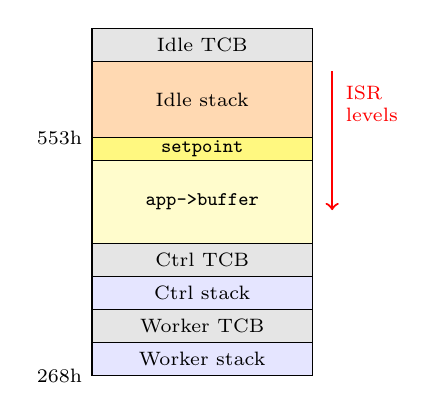
\begin{tikzpicture}[x=1cm,y=0.42cm,font=\scriptsize]
      \draw[fill=blue!10] (0,0) rectangle (2.8,1) node[midway]{Worker stack};
      \draw[fill=gray!20] (0,1) rectangle (2.8,2) node[midway]{Worker TCB};
      \draw[fill=blue!10] (0,2) rectangle (2.8,3) node[midway]{Ctrl stack};
      \draw[fill=gray!20] (0,3) rectangle (2.8,4) node[midway]{Ctrl TCB};
      \draw[fill=yellow!20] (0,4) rectangle (2.8,6.5) node[midway]{\texttt{app->buffer}};
      \draw[fill=yellow!50] (0,6.5) rectangle (2.8,7.2) node[midway]{\texttt{setpoint}};
      \draw[fill=orange!30] (0,7.2) rectangle (2.8,9.5) node[midway]{Idle stack};
      \draw[fill=gray!20] (0,9.5) rectangle (2.8,10.5) node[midway]{Idle TCB};
      \draw[->,red,thick] (3.05,9.2) -- (3.05,5);
      \node[red,right,align=left] at (3.1,8.2) {ISR\\levels};
      \node[left] at (0,0) {268h};
      \node[left] at (0,7.2) {553h};
    \end{tikzpicture}
    \end{column}
    \begin{column}{0.62\textwidth}
      \small
      Long work, switch~2 OFF (nesting):
      \begin{itemize}
        \item \textbf{2\,ms:} depth 2, both levels on the Idle stack, 27 bytes each.
        \item \textbf{8\,ms:} level 8 overwrites \texttt{app->setpoint}. FreeRTOS does not notice.
        \item \textbf{16\,ms:} next tick, switch from Idle to Ctrl. Only now \texttt{configCHECK\_FOR\_STACK\_OVERFLOW} compares Idle's saved SP with the start of its stack: about 250 bytes below $\Rightarrow$ \texttt{vApplicationStackOverflowHook}.
      \end{itemize}
      Long work, switch~2 ON (deferred):
      \begin{itemize}
        \item Depth stays 1, all stacks flat. The Worker cannot keep up: \texttt{ulTaskNotifyTake()} returns 2 or 3 pending ticks $\Rightarrow$ counted as overruns.
      \end{itemize}
    \end{column}
  \end{columns}
\end{frame}

\scriptonly{%
The debug setup of example~9 adds two views to the Debug Console. \texttt{-exec tasks} lists every task with its priority, the start of its stack (\texttt{pxStack} in the TCB) and its current stack pointer: for the running task the CPU register SP, for all others the value saved in the TCB at the last switch. The difference is the number of bytes the task has left; a negative value is an overflow. \texttt{-exec heap} lists the heap blocks in address order. At the breakpoint \texttt{dbgRtosStackOverflow} the Idle task has $-256$ bytes left, while the stacks of all other tasks are untouched.

The check of FreeRTOS runs only when a task is switched out, and method~1 only compares the saved stack pointer with the start of the stack. Between two checks the overflow is invisible, and the overflow can destroy the data the check needs: with a smaller \texttt{app} block the stack reaches the TCB of Ctrl before the next tick. Ctrl is then no longer woken, there is no task switch, and in the simulation the hook was called only after 258\,ms, after the stack had passed through the TCBs and stacks of two more tasks. The check is a useful alarm, not a protection. The design rule is the one of example~6: every task stack must have room for its own worst case \emph{plus} the deepest ISR frame, and that depth has a bound only if ISRs do not nest themselves. Moving the work into a task (switch~2) gives this bound. The load problem remains, but it shows up as counted overruns and a starved Ctrl task instead of as corrupted memory.
}

% ===========================================================================
\section{Static Code Analysis}
\label{sec:static}

\begin{frame}{Static code analysis}
  \begin{itemize}
    \item The code itself is analysed, usually the \emph{object code}: the machine instructions that actually run.
    \item Cycles per instruction $\rightarrow$ per basic block $\rightarrow$ longest path through the control flow graph, with a bound for every loop.
    \item Execution time $T_{SA} = \text{cycles}_{max} / f_{\text{machine cycle}}$.
    \item With safety requirements: the code must not be changed after the analysis (and the compiler settings neither).
    \item Safety margin factor $c = 2 \dots 3$: \quad $T_{V,max} \le c \cdot T_{SA}$.
    \item The same method gives the maximum \emph{stack} usage.
  \end{itemize}
\end{frame}

\begin{frame}{Example 5: WCET of the ISR}
  \small
  \begin{tabular}{@{}lll@{}}
    \toprule
    Block & Instructions & Cycles \\
    \midrule
    Vectoring (hardware call) & -- & 2 \\
    Entry & \texttt{LJMP}, 2$\times$\texttt{PUSH}, \texttt{MOV PSW}, \texttt{INC}, \texttt{MOV R7}, \texttt{JB} & 12 \\
    Long branch & \texttt{MOV R7,\#NLONG} & 1 (short: 0) \\
    Call and return & \texttt{CALL}, \texttt{RET} & 4 \\
    Loop (bound $N$) & \texttt{DJNZ} & $2N$ \\
    Overrun check & \texttt{JNB}, \texttt{INC} & 3 (no overrun: 2) \\
    Exit & 2$\times$\texttt{POP}, \texttt{RETI} & 6 \\
    \midrule
    \multicolumn{2}{@{}l}{Longest path} & $2N + 28$ \\
    \bottomrule
  \end{tabular}
  \medskip
  \begin{itemize}
    \item $N = 230$: $C = 488$\,\textmu s, $\rho = 488/200 = 2.44$ $\Rightarrow$ not schedulable.
    \item $N = 40$: $C = 106$\,\textmu s, $\rho = 0.53$. Plus response latency $\le 9$\,\textmu s.
    \item Largest $N$: the next tick must not arrive before the ISR has finished. Latency up to 9 cycles, 2 of them already in $C$: $2N + 28 + 7 \le 200 \Rightarrow N \le 82$. With $c = 2$: $2(2N+28) \le 200 \Rightarrow N \le 36$.
  \end{itemize}
\end{frame}

\scriptonly{%
The analysis needs exactly the information that is in the right-hand column of Example~\ref{lst:ex05}: the cycles of each instruction, the structure of the branches, and a bound for each loop. The loop bound is the critical input; here it is the constant loaded into R7. Whoever reads the analysis must be sure that no other path can load a larger value, which is why the code may not change afterwards. The response latency of up to 9 machine cycles is not part of $C$ but adds to the reaction time $T_R$, as do the interrupt-disabled sections of the main program.
}

\begin{frame}{Static stack analysis}
  \begin{itemize}
    \item Call graph with the stack usage of each function. Worst case = deepest path from \texttt{main} + deepest path of each ISR priority level.
    \item Example 5: \texttt{main} 0 bytes. \texttt{t0isr}: PC 2 + PSW, ACC 2 + call of \texttt{work} 2 $= 6$ bytes $\Rightarrow$ SP $\le$ 2Fh + 6 = 35h. Proven bound.
    \item Example 6: the ISR enables its own level again $\Rightarrow$ edge from \texttt{t0isr} to itself, like recursion. The depth depends on timing; without a proof of $C < T$ the stack has no bound $\Rightarrow$ rejected.
    \item Rules that make the analysis possible: no recursion (MISRA C), no re-enabling of interrupts inside an ISR, no dynamic stack allocation.
  \end{itemize}
\end{frame}

\begin{frame}{Limits and tools}
  \begin{itemize}
    \item Simple microcontrollers (8051, AVR): fixed cycles per instruction, analysis by hand is feasible for small sections.
    \item Pipelines, caches, and branch prediction: the cycle count depends on history $\Rightarrow$ tools with a hardware model, e.g.\ AbsInt aiT (WCET) and StackAnalyzer, OTAWA (open source).
    \item GCC: \texttt{-fstack-usage} (stack per function), \texttt{-Wstack-usage=}$n$; \texttt{avr-objdump -d} shows the instructions to count.
    \item Static analysis gives a safe upper bound, measurement gives a value that was actually reached. Use both: the measured maximum must lie below the static bound.
  \end{itemize}
\end{frame}

\subsection{Exercise}
\begin{frame}{Exercise: EdSim51 (1/2)}
  \begin{enumerate}
    \item \textbf{Trace.} Enter the four instructions of the tracing example in EdSim51, step through them, and record PC, A, and PSW after each step.
    \item \textbf{Prediction.} For example~5 compute $C$ and $\rho$ for both positions of SW0. Predict TICKS, OVERRUN, and MAINHI after 20\,ms.
    \item \textbf{Measurement.} Run example~5 in both positions and compare. Where does the main loop stand after each ISR with the long work?
    \item \textbf{Limit.} Change \texttt{NLONG} to 82, 85, and 86. Check your static bound with the OVERRUN counter. Why does 86 already give overruns although $2N + 28 = 200$?
  \end{enumerate}
\end{frame}

\begin{frame}{Exercise: EdSim51 (2/2)}
  \begin{enumerate}
    \setcounter{enumi}{4}
    \item \textbf{Stack.} Run example~6 with short work in single steps through one ISR. Write down the 7 stack bytes and explain each.
    \item \textbf{Overflow.} Switch to long work. At which tick is SETPOINT overwritten, by which byte, and at which tick does the guard stop the program? Compare with $d(t)$.
    \item \textbf{Reset value.} Remove \texttt{MOV SP,\#2FH} from example~5. Which bytes does the stack overwrite now?
    \item \textbf{Redesign.} Move the work out of the ISR: the ISR only sets a flag, the main loop does the work. What happens to the lost ticks now, and how would you detect them?
  \end{enumerate}
\end{frame}

\scriptonly{%
Hints. In exercise~4 the ISR does not start at the overflow: the current instruction of the main loop finishes first, then the hardware call follows. With $C = 199$ cycles (no overrun increment) the ISR and one main instruction no longer fit into 200 cycles, the start drifts later with every tick until TF0 is set before the check. The static bound $N \le 82$ covers the worst-case latency, $N = 85$ only works because the main loop contains no long instructions. In exercise~7 the stack starts at 08h, in register bank~1, which the ISR uses as R0--R7. Check whether R7 of bank~1 (0Fh) is hit. In exercise~8 the work is still longer than the period; the difference is \emph{where} the problem appears and whether it can be counted.
}
